% \chapter{Mạng Neural hồi quy - Recurrent Neural Network}

\section{Giới thiệu về RNN}
% \subsection{Vấn đề của mạng thường với dữ liệu sequence}

\subsection{Ý tưởng cơ bản của RNN}
Recurrent Neural Networks (RNNs), hay mạng neural hồi quy, là một kiến trúc neural network mà ở đó, trạng thái của mô hình tại bước liền trước sẽ được dùng làm đầu vào của bước hiện tại. Nói cách khác, một mô hình RNN sẽ hoạt động theo dạng ánh xạ dữ liệu đầu vào và trạng thái trước đó của mô hình thành dữ liệu đầu ra.

\begin{figure}[!h]
    \centering
    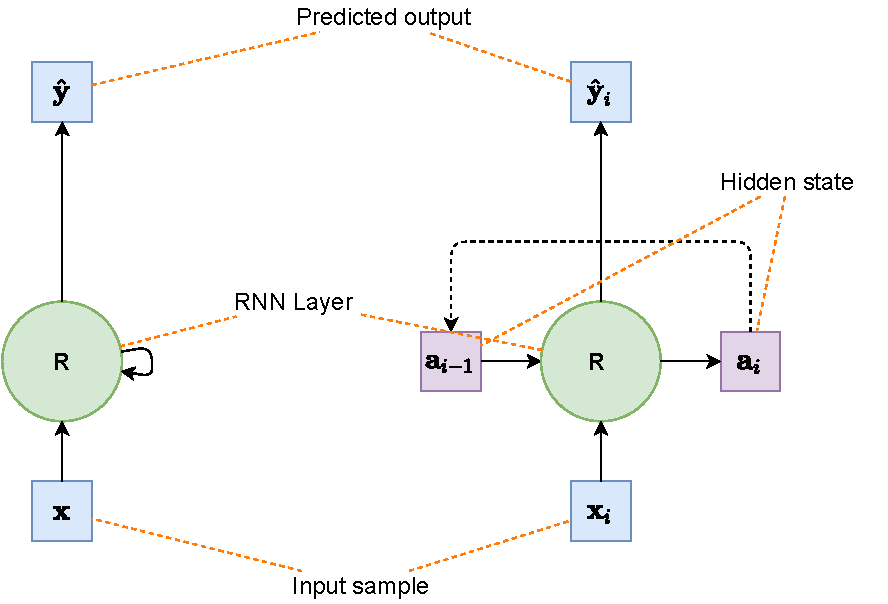
\includegraphics[width=\textwidth,height=\textheight,keepaspectratio]{books/artificial-neural-network/chapter06/figure-sec2345/rnn.pdf}
    \caption{Kiến trúc của một lớp RNN. \emph{Bên trái:} biểu diễn với đường nối vòng. \emph{Bên phải:} Biểu diễn với hidden state}
\end{figure}

Với mạng neural truyền thống dạng feed-forward, dữ liệu chỉ được truyền theo một chiều, tính toán và đưa ra kết quả gói gọn trong một pha dựa hoàn toàn vào dữ liệu input (không tồn tại đường nối vòng). Ta cần làm rõ rằng đường nối vòng ở đây không tạo ra một chu kì tính toán lặp lại vô hạn, mà chỉ dùng dữ liệu từ pha tính toán trước làm đầu vào cho pha hiện tại. Cụ thể hơn, ta "gỡ" đường nối vòng (unfold) để đưa ra kiến trúc tính toán cụ thể hơn khi truyền dữ liệu sequence vào mạng:

\begin{figure}[!h]
    \centering
    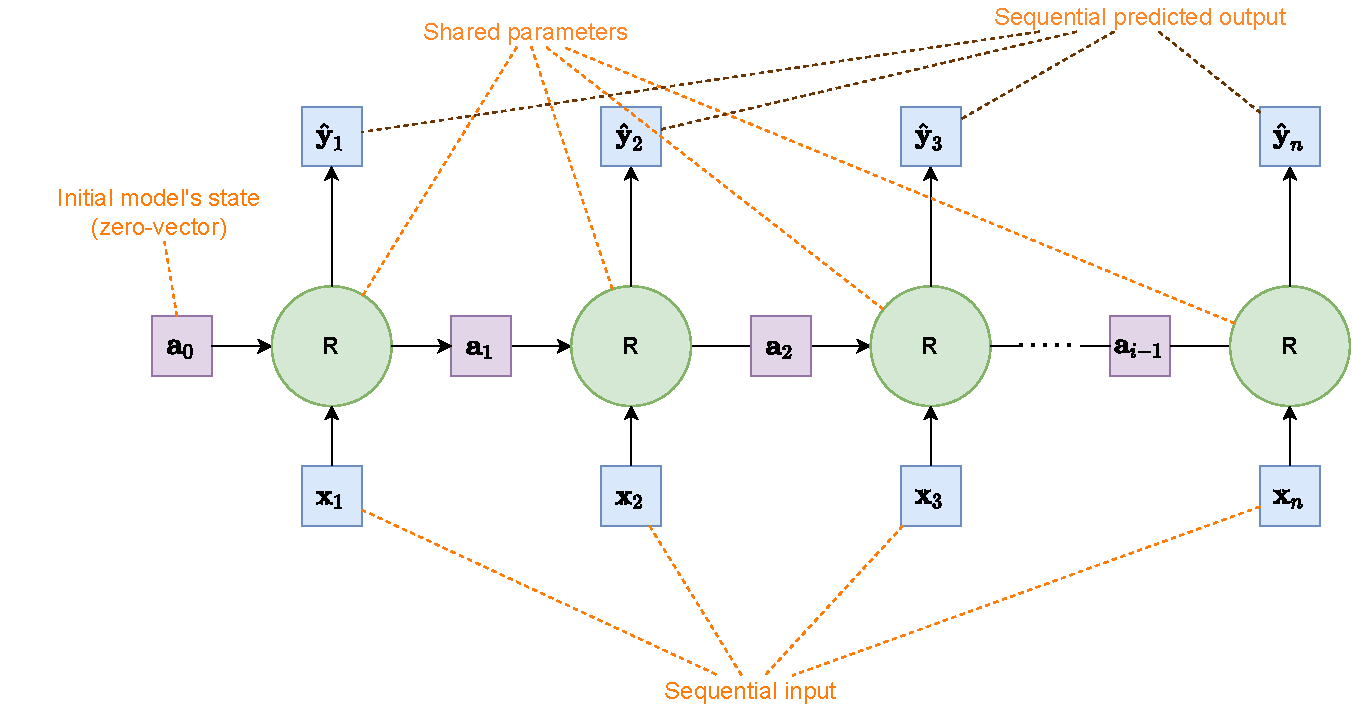
\includegraphics[width=\textwidth,height=\textheight,keepaspectratio]{books/artificial-neural-network/chapter06/figure-sec2345/unfold_rnn.pdf}
    \caption{Luồng tính toán cụ thể trên sequence của RNN}
\end{figure}

Với RNN, việc thông tin từ lần truyền trước được lưu lại (tại hidden state) cho lần tính toán hiện tại, tạo ra một đường nối vòng trên đồ thị tính toán. Nói cách khác, hidden state đóng vai trò như một bộ nhớ của lớp RNN. Điều này đặc biệt hữu dụng khi xử lý dữ liệu dạng sequence, khi ta có thể áp dụng cùng một logic tính toán (cùng cách tính và bộ trọng số) cho từng điểm dữ liệu trong chuỗi, giữ được thông tin từ các điểm trước đó, đồng thời vẫn giữ được thông tin về thứ tự của sequence.

Năm 1982, Hopfield đã đưa ra kiến trúc Hopfield network là một dạng mạng neural với khả năng lưu giữ lại trạng thái cũ trước đó để hỗ trợ cho lần tính toán hiện tại. Hopfield network là một dạng đặc biệt của RNN. Trọng số trên mạng Hopfield được cập nhật bằng phương pháp tối ưu lồi (khác với gradient descent ở RNN hiện đại). RNN chính thức được đưa ra dựa trên công trình của David Rumelhart năm 1986.

Hiển nhiên ta không thể áp dụng cùng một kiến trúc RNN nêu trên cho mọi bài toán với dữ liệu sequence. Một số mẫu biến thể thiết kế (design patterns) từ kiến trúc trên để áp dụng cho từng loại bài toán:
\begin{figure}[!h]
    \centering
    \label{rnn_genre}
    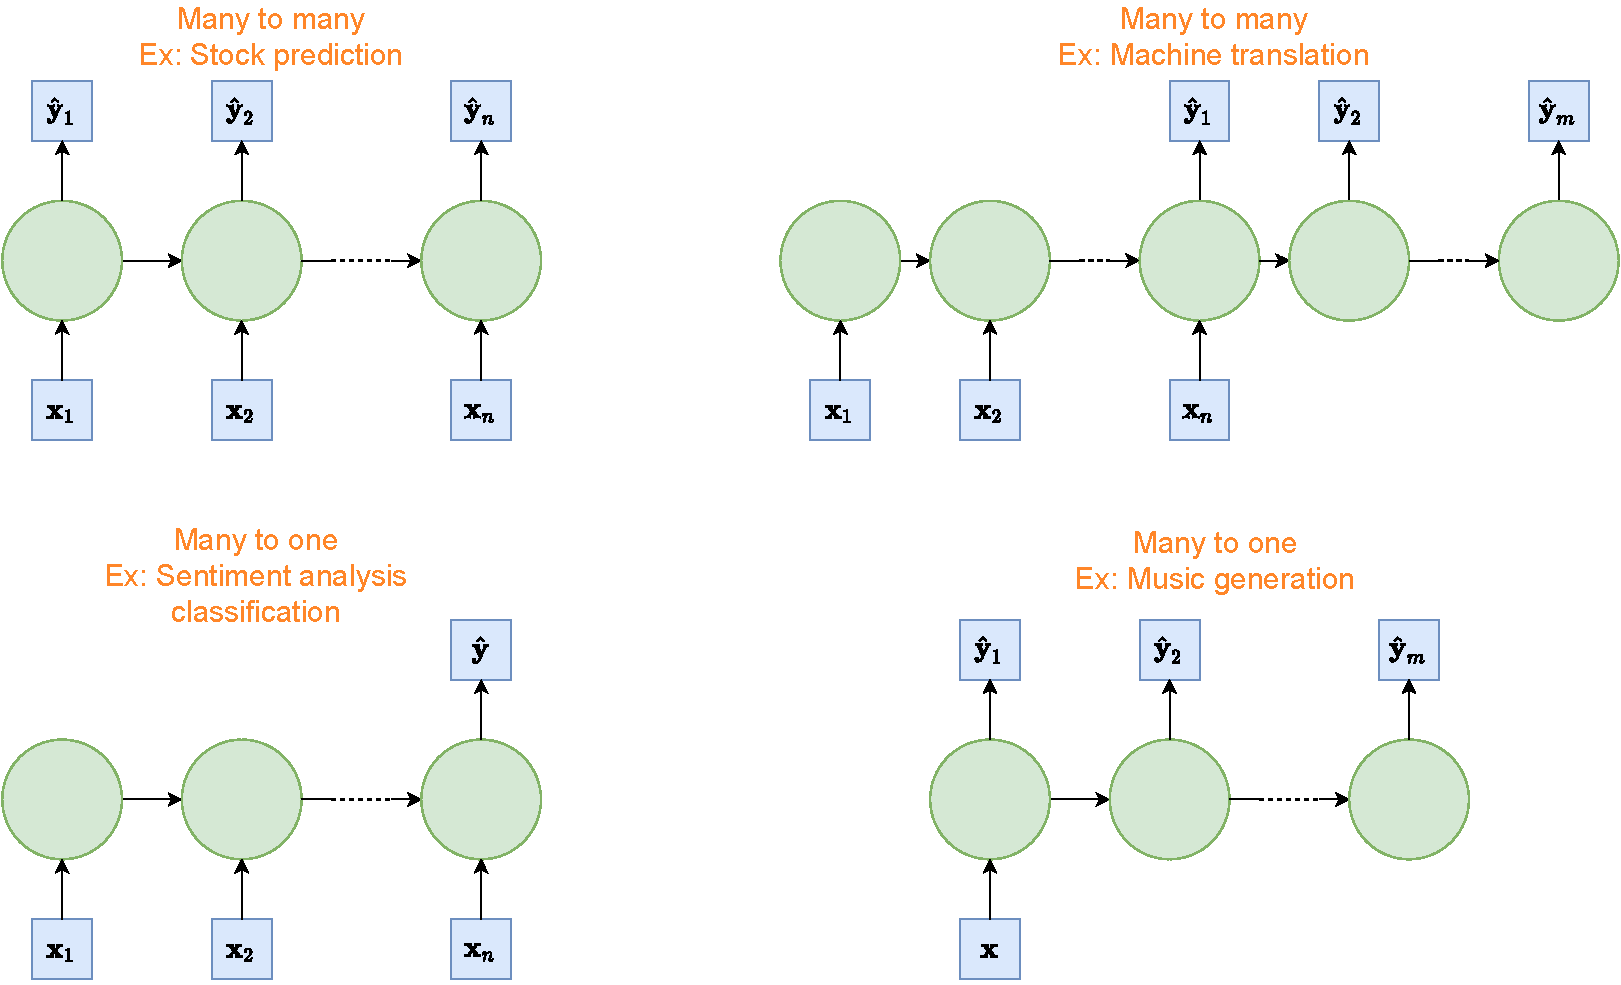
\includegraphics[width=\textwidth,height=\textheight,keepaspectratio]{books/artificial-neural-network/chapter06/figure-sec2345/rnn_genre.pdf}
    \caption{Các mẫu thiết kế RNN cho từng loại bài toán}
\end{figure}

\section{Cơ chế lan truyền xuôi của RNN}
Để tìm hiểu rõ hơn cách hoạt động cụ thể của RNN, mục này sẽ trình bày cơ chế để lan truyền một sequence dữ liệu qua mạng. Ta xét kiến trúc mạng cụ thể cơ bản của RNN, được biểu diễn dưới dạng công trức truy hồi như sau (lưu ý vector được biểu diễn dưới dạng cột):
\begin{align}
     & \symbf a_0 = 0              \\ \nonumber
     & \symbf a_i = f (\textbf W_{ax}\cdot \textbf x_i + \textbf W_{aa} \cdot \textbf a_{i-1} + \textbf b_a) \\ \nonumber
     & \symbf{\hat{y_i}} = g(\textbf W_{ya} \cdot \textbf a_i + \textbf b_y) \label{rnn_equation}
\end{align}

Các biến số và tham số trong công thức truy hồi trên được định nghĩa là:
\begin{itemize}
    \item $\symbf a_i$ là hidden state - trạng thái ẩn của mô hình. $\symbf a_0 = 0$ là quy ước cho trạng thái bắt đầu.
    \item $\symbf{\hat{y_i}}$ là giá trị dự đoán đầu ra ứng với bước $i$.
    \item $\symbf x_i$ là giá trị đầu vào tại bước $i$.
    \item $f$ và $g$ là các hàm activation phù hợp. Thông thường, ta chọn $f(x) = \tanh(x)$ hoặc $f(x) = \textrm{ReLU}(x)$ và $g(x) = \sigma (x)$ hoặc $g(x) = \textrm{Softmax(x)}$, tùy vào cách thiết kế và yêu cầu bài toán.
    \item $\textbf W$ và $\textbf b$ là các trọng số của mô hình, cụ thể:
          \begin{itemize}
              \item $\textbf W_{ax}$ là ma trận của phép ánh xạ tuyến tính biến đổi $\textbf x$ thành một thành phần trong $\textbf a$
              \item $\textbf W_{aa}$ là ma trận của phép ánh xạ tuyến tính biến đổi trạng thái $\textbf a$ cũ thành một thành phần trong trạng thái $\textbf a$ mới.
              \item $\textbf b_a$ là bias của phép biến đổi tìm $\textbf a$
              \item $\textbf W_{ya}$ là ma trận của phép ánh xạ tuyến tính biến đổi trạng thái hiện tại $\textbf a$ thành kết quả đầu ra $\hat{\textbf{y}}$
              \item $\textbf b_a$ là bias của phép biến đổi tìm $\hat{\textbf{y}}$
          \end{itemize}
\end{itemize}
Ở dạng đồ thị tính toán, một nút RNN cơ bản có thể được biểu diễn bằng:
\begin{figure}[H]
    \centering
    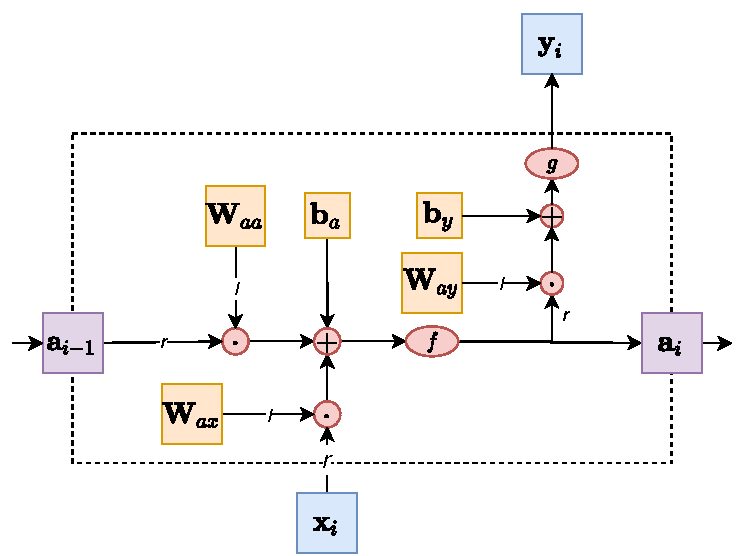
\includegraphics[width=\textwidth,height=\textheight,keepaspectratio]{books/artificial-neural-network/chapter06/figure-sec2345/rnn_elman.pdf}
    \caption{Đồ thị tính toán cụ thể của một nút trong RNN}
\end{figure}

Về lý thuyết, với mỗi nút đầu vào của sequence, RNN sẽ đều cho ra một kết quả đầu ra. Tuy nhiên, chọn nút đầu ra nào làm kết quả và tối ưu như thế nào là tùy vào mục tiêu của bài toán. Lấy ví dụ trong các trường hợp sau:
\begin{itemize}
    \item Với bài toán dự đoán giá cổ phiếu (dạng many-to-many đối xứng): Giả sử chuỗi sequence là thông tin input của mạng theo từng ngày và đầu ra của mạng là giá cổ phiếu cho ngày hôm đó. Với cách thiết kế many-to-many, mỗi $\hat{\textbf{y}}$ đều tương ứng với một ngày nào đó trong sequence. Vì vậy, mọi đầu ra tại từng bước đều mang ý nghĩa. Ta cần tính toán hàm loss dựa trên tất cả giá trị đầu ra của mạng.
    \item Với bài toán sentiment classification (dạng many-to-one): xét trường hợp đơn giản nhất là gắn một nhãn tốt/xấu cho một câu, với dữ liệu đầu vào là từng từ trong câu đó, đầu ra là kết quả dữ đoán câu đó tốt hay xấu. Vì mỗi câu chỉ mang duy nhất một nhãn, ta nhận thấy rằng, chỉ có kết quả dự đoán của mô hình khi toàn bộ câu đã được truyền vào mới mang ý nghĩa.
          \begin{itemize}
              \item Câu "This movie is not bad" khi được truyền toàn bộ vào model, model có thể gắn nhãn "tốt" cho câu (phim không tệ là phim hay)
              \item Tuy nhiên, cùng với câu trên, khi chỉ lấy đoạn "This movie is not", model lại có thể gắn nhãn "xấu" cho câu (từ "not" mang nghĩa phủ định, có thể là tiêu cực)
          \end{itemize}
          Lẽ dĩ nhiên, qua mỗi bước truyền, mạng đều cho ra một kết quả đánh giá mức tốt/xấu của câu đến điểm đó. Tuy nhiên, xét riêng trong ngữ cảnh bài toán này, ta quan tâm tới nhãn của toàn câu chứ không quan tâm nhãn của từng đoạn ngắn trong câu. Vì vậy, chỉ có output ở nút cuối cùng là có ý nghĩa.
\end{itemize}

Việc xác định cụ thể ta cần chọn đầu ra nào là rất quan trọng, vì mô hình sẽ dựa vào đúng đầu ra có ý nghĩa đó để cập nhật trọng số. Việc lan truyền của RNN có thể được hiểu thông qua hiện thực cụ thể ở đoạn code sau (python):
\begin{python}
    import numpy as np

    dim_x = 5  # Input dimension
    dim_y = 5  # Output dimension
    dim_a = 3  # Hidden state dimension

    n = 10  # Input sequence length

    X = np.random.randn(n, dim_x)

    W_ax = np.random.rand(dim_a, dim_x)  # Shape(W_ax) = (3, 5)
    W_aa = np.random.rand(dim_a, dim_a)  # Shape(W_aa) = (3, 3)
    b_a = np.random.rand(dim_a)          # Shape(b_a)  = (3,)
    W_ya = np.random.rand(dim_y, dim_a)  # Shape(W_ya) = (5, 3)
    b_y = np.random.rand(dim_y)          # Shape(b_y)  = (5,)

    a = np.zeros(dim_a)  # Initial state = zeros
    y = []

    # Forwarding process
    for i in range(n):
        xi = X[i].T  # Transform into column-vector
        # Follow equation 2.1 with f is tanh and g is softmax
        a = np.tanh(np.dot(W_ax, xi) + np.dot(W_aa, a) + b_a)
        yi = np.dot(W_ya, a) + b_y
        yi = np.exp(yi) / np.sum(np.exp(yi))
        y.append(yi)
\end{python}

\section{Cơ chế lan truyền ngược của RNN}
Nhắc lại về các bước huấn luyện một mạng feed-forward với gradient descent:
\begin{enumerate}
    \item Bước forward: Đưa dữ liệu đầu vào $\textbf x$ qua mạng, thu được kết quả đầu ra $\hat{\textbf{y}}$
    \item Tính toán hàm loss $\mathcal{L}(\hat{\textbf{y}})$ cho bài toán unsupervised learning hoặc $\mathcal{L}(\hat{\textbf{y}},\textbf y)$ cho bài toán supervised
    \item Bước backward: Tính đạo hàm của hàm loss $\Delta w = \delta \mathcal{L} / \delta w$ cho từng tham số $w$ trong mạng
    \item Bước cập nhật: Cập nhật các tham số theo learning rate $\alpha$ hiện tại: $w \leftarrow w - \alpha\Delta w$
\end{enumerate}

Quá trình này cũng tương tự với RNN. Tuy nhiên, vì tính đặc thù với đường nối vòng, một số vấn đề sẽ nảy sinh khiến ta cách tối ưu thông thường gặp phải nhiều vấn đề. Ta xét một mạng RNN với hàm loss dạng cũ và dữ liệu dạng supervised như hình:
\begin{figure}[!h]
    \centering
    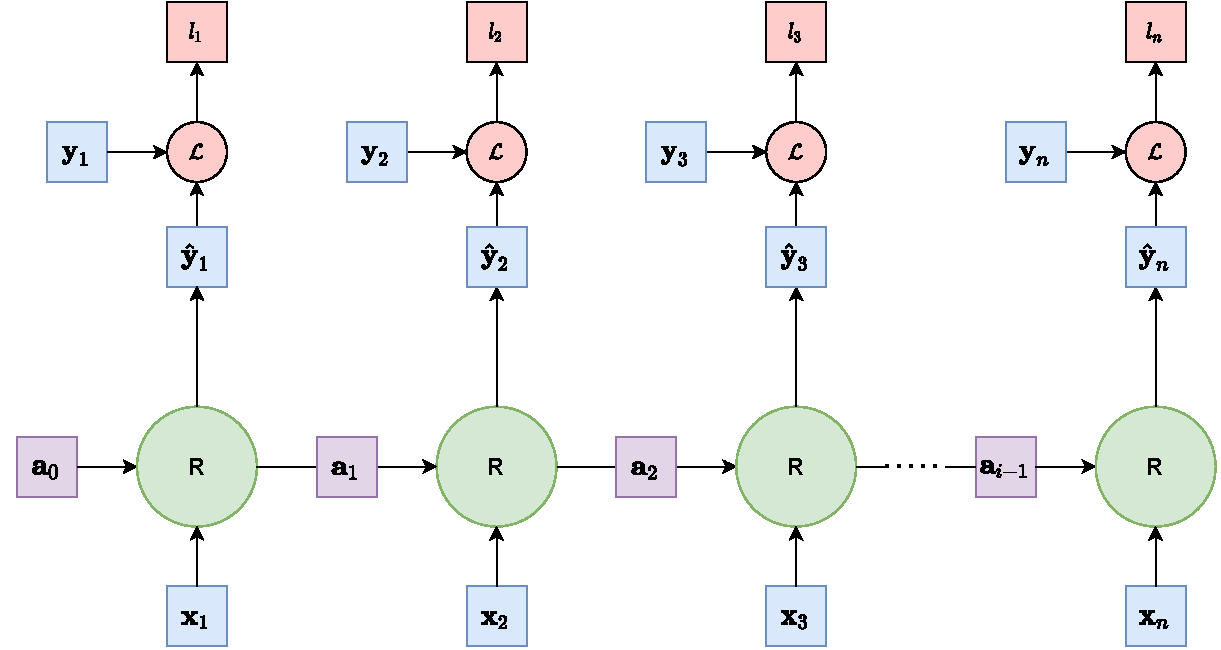
\includegraphics[width=\textwidth,height=\textheight,keepaspectratio]{books/artificial-neural-network/chapter06/figure-sec2345/rnn_with_loss.pdf}
    \caption{RNN với hàm loss}
\end{figure}

Với kiến trúc truyền tuần tự từng mẫu, tại mỗi thời điểm, chúng ta đều tính toán được một giá trị đầu ra. Hàm loss truyền thống tính toán được giá trị hàm loss dựa trên một giá trị đầu ra dự báo $\hat{\textbf{y}}$ và một giá trị nhãn thực $\textbf y$, nên với hướng tiếp cận này, chúng ta có nhiều hơn một giá trị hàm loss tại mỗi bước. Tuy nhiên, để thực hiện tính toán đạo hàm truyền ngược, ta cần một giá trị loss duy nhất. Vì vậy, ta cần một hàm loss mới, nhận giá trị đầu vào là tất cả các đầu ra của mạng $\hat{\textbf{y}}_i$ và tất cả các nhãn ở từng bước $\textbf y$, và cho ra một con số duy nhất là hàm mất mát của toàn bộ quá trình. Một số hướng tiếp cận để giải quyết vấn đề này như:
\begin{itemize}
    \item Với bài toán dạng many-to-one: Ta chỉ quan tâm đến một giá trị đầu ra cuối cùng của mạng. Vì vậy, ta chỉ cần tối ưu nhãn cuối cùng của một pha: $\mathcal{L} = \mathcal{L}(\hat{\textbf{y}}_n,\textbf y_n)$
    \item Với các bài toán còn lại: khi có nhiều hơn một output, ta có thể chọn một hàm để tích hợp các giá trị $l_i$ lại thành một giá trị duy nhất (tổng, trung bình, max, etc) tùy vào trường hợp bài toán cụ thể.
\end{itemize}

Để nhìn nhận quá trình một cách rõ ràng hơn, vì tất cả các nút RNN đều chia sẻ trọng số trong quá trình đưa từng mẫu dữ liệu qua mạng, ta tách trọng số của mô hình ra thành các khối dữ liệu. Khi đó, mô hình bao gồm cả hàm loss sẽ có dạng:
\begin{figure}[!h]
    \centering
    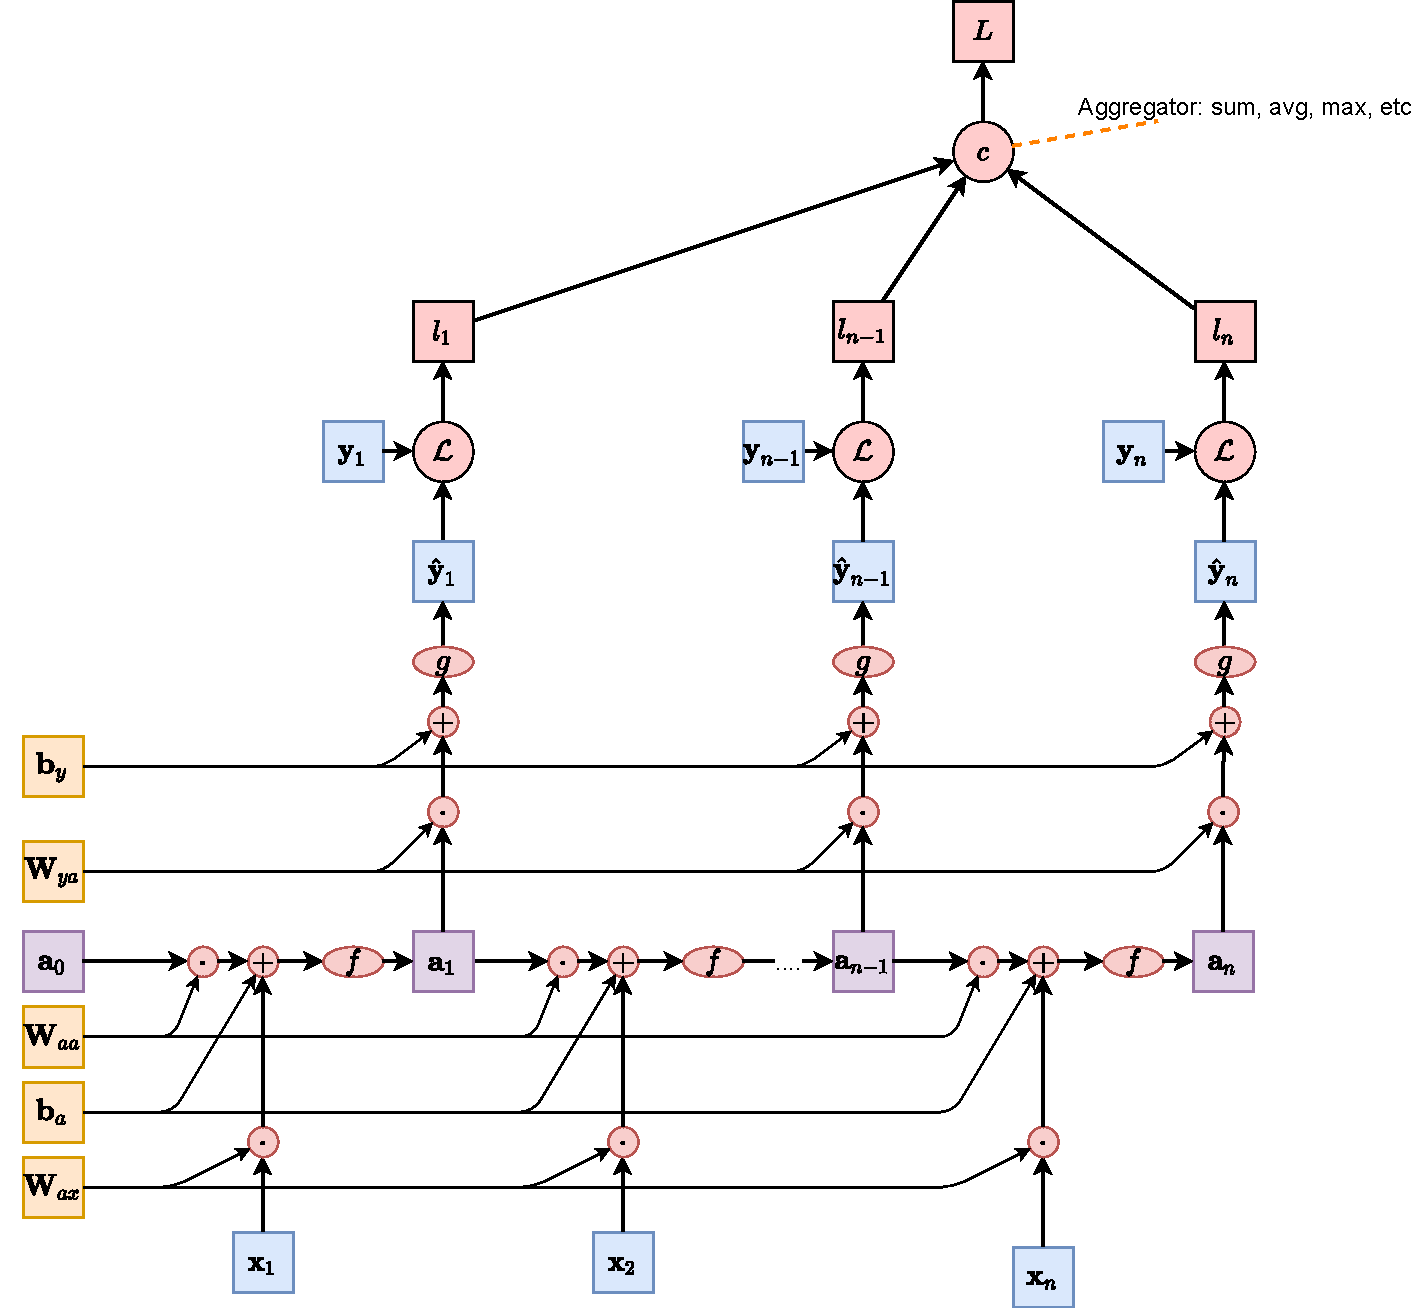
\includegraphics[width=\textwidth,height=\textheight,keepaspectratio]{books/artificial-neural-network/chapter06/figure-sec2345/rnn_backprop.pdf}
    \caption{RNN với hàm loss và trọng số cụ thể}
\end{figure}

với các thành phần mới:
\begin{itemize}
    \item $l_i = \mathcal{L}(\hat{\symbf{y}}_i, \symbf{y}_i)$ là giá trị hàm loss cho đầu ra thứ $i$
    \item $L = c(l_1,l_2,...,l_n)$ là giá trị hàm loss tổng; $c$ là một hàm tích hợp nhiều giá trị loss (tổng, max, etc)
\end{itemize}

Với sự hỗ trợ của các framework tính toán hiện đại, việc tính toán đạo hàm hầu hết đã được tự động hóa. Tuy nhiên, để nắm rõ quy trình hoạt động của RNN cũng như đánh giá khả năng hoạt động của kiến trúc, phần này sẽ trình bày cụ thể cách tính đạo hàm trong RNN.

Ta tính lần lượt các giá trị $\Delta w = \frac{\partial L}{\partial w}$ cho từng tham số $w$ trong mạng, cụ thể là từng bộ tham số $\symbf W_{ya}, \symbf b_y, \symbf W_{aa}, \symbf W_{ax}, \symbf b_a$:

    $$\Delta \symbf W_{ya} = \frac{\partial L}{\partial \symbf W_{ya}}  = \sum_{i=1}^{n}\left(
        \frac{\partial L}{\partial l_i} \cdot
        \frac{\partial l_i}{\partial \hat{\symbf y}_i} \cdot
        \frac{\partial \hat{\symbf y}_i}{\partial \symbf W_{ya}}
     \right) = \sum_{i=1}^{n}\left(
        \frac{\partial L}{\partial l_i} \cdot
        \frac{\partial l_i}{\partial \hat{\symbf y}_i} \cdot
        g'(\symbf W_{ya}\cdot\symbf a_i + \symbf b_y) \cdot
        \frac{\partial (\symbf W_{ya}\cdot\symbf a_i)}{\partial \symbf W_{ya}}
     \right)$$

     $$\Delta \symbf b_y = \frac{\partial L}{\partial \symbf b_y}  = \sum_{i=1}^{n}\left(
        \frac{\partial L}{\partial l_i} \cdot
        \frac{\partial l_i}{\partial \hat{\symbf y}_i} \cdot
        \frac{\partial \hat{\symbf y}_i}{\partial \symbf b_y}
     \right) = \sum_{i=1}^{n}\left(
        \frac{\partial L}{\partial l_i} \cdot
        \frac{\partial l_i}{\partial \hat{\symbf y}_i} \cdot
        g'(\symbf W_{ya}\cdot\symbf a_i + \symbf b_y)
     \right)$$

     $$\Delta \symbf W_{aa} = \frac{\partial L}{\partial \symbf W_{aa}}  = \sum_{i=1}^{n}\left(
        \frac{\partial L}{\partial l_i} \cdot
        \frac{\partial l_i}{\partial \hat{\symbf y}_i} \cdot
        \frac{\partial \hat{\symbf y}_i}{\partial \symbf a_i} \cdot
        \frac{\partial \symbf a_i}{\partial \symbf W_{aa}}
     \right) = \sum_{i=1}^{n}\left(
        \frac{\partial L}{\partial l_i} \cdot
        \frac{\partial l_i}{\partial \hat{\symbf y}_i} \cdot
        \symbf W_{ya} \cdot \text P_i
     \right)$$
     với
     $$\text P_i = \frac{\partial \symbf a_i}{\partial \symbf W_{aa}} = f_i' \cdot \left(\symbf W_{aa}  + \symbf I \right)\cdot \frac{\partial \symbf a_{i-1}}{\partial \symbf b_a} = f_i' \cdot \left(\symbf W_{aa}  + \symbf I \right)\cdot \text P_{i-1} \quad ;\quad  \text P_0 = 0 $$

     $$\Delta \symbf b_a = \frac{\partial L}{\partial \symbf W_{ya}}  = \sum_{i=1}^{n}\left(
        \frac{\partial L}{\partial l_i} \cdot
        \frac{\partial l_i}{\partial \hat{\symbf y}_i} \cdot
        \frac{\partial \hat{\symbf y}_i}{\partial \symbf a_i} \cdot
        \frac{\partial \symbf a_i}{\partial \symbf b_a}
     \right) = \sum_{i=1}^{n}\left(
        \frac{\partial L}{\partial l_i} \cdot
        \frac{\partial l_i}{\partial \hat{\symbf y}_i} \cdot
        \symbf W_{ya} \cdot \text Q_i
     \right)$$
     với
     $$\text Q_i = \frac{\partial \symbf a_i}{\partial \symbf b_a} = f_i' \cdot \left(\symbf W_{aa} \cdot \frac{\partial \symbf a_{i-1}}{\partial \symbf b_a} + \symbf I \right) = f_i' \cdot \left(\symbf W_{aa} \cdot \text Q_{i-1} + \symbf I \right)\quad ;\quad \text Q_0 = 0 $$

     $$\Delta \symbf W_{ax} = \frac{\partial L}{\partial \symbf W_{ax}}  = \sum_{i=1}^{n}\left(
        \frac{\partial L}{\partial l_i} \cdot
        \frac{\partial l_i}{\partial \hat{\symbf y}_i} \cdot
        \frac{\partial \hat{\symbf y}_i}{\partial \symbf a_i} \cdot
        \frac{\partial \symbf a_i}{\partial \symbf W_{ax}}
     \right) = \sum_{i=1}^{n}\left(
        \frac{\partial L}{\partial l_i} \cdot
        \frac{\partial l_i}{\partial \hat{\symbf y}_i} \cdot
        \symbf W_{ya} \cdot \text R_i
     \right)$$
     với
     $$\text R_i = \frac{\partial \symbf a_i}{\partial \symbf W_{ax}} = f_i' \cdot \left(\frac{\partial (\symbf W_{ax}\cdot \symbf x_i)}{\partial \symbf W_{ax}} + \symbf W_{aa} \cdot \frac{\partial \symbf a_{i-1}}{\partial \symbf W_{ax}}\right) = f_i' \cdot \left(\frac{\partial (\symbf W_{ax}\cdot \symbf x_i)}{\partial \symbf W_{ax}} + \symbf W_{aa} \cdot R_{i-1}\right) \quad ;\quad  \text R_0 = 0 $$

Bạn đọc có thể tự chứng minh các biểu thức đạo hàm ở trên (Dựa vào đồ thị tính toán, đạo hàm của một nút dữ liệu bất kì $b$ theo một nút $a$ bằng tổng đạo hàm theo chain rule trên tất cả các đường đi từ $a$ đến $b$).\\
Với RNN, trên đồ thị tính toán, có nhiều hơn một đường đi từ một nút tham số bất kì tới nút hàm mục tiêu $\mathcal{L}$. Có thể nhận xét rằng đường nối vòng trong RNN làm việc tính toán đạo hàm thủ công trở nên phức tạp hơn so với trên mạng feed-forward truyền thống.

% \section{Quá trình huấn luyện cho mạng RNN }
% Appendix
\section{Ưu và nhược điểm của RNN}
RNN được thiết kế đặc thù để giải quyết dữ liệu dạng sequence. Một số ưu điểm của RNN so với mạng feed-forward kiểu truyền thống có thể kể đến như:
\begin{itemize}
    \item Khả năng xử lý dữ liệu với độ dài bất định
    \item Kích thước mô hình là cố định và độc lập với độ dài đầu vào
    \item Việc tính toán có tận dụng được thông tin từ quá khứ
    \item Sử dụng chung một bộ trong số cho toàn bộ sequence, tức áp dụng cùng một logic tính toán trên từng điểm dữ liệu trong sequence.
    \item Chia sẻ trọng số trong quá trình tính toán còn giúp làm giảm số lượng tham số, cải thiện tính tổng quát hóa (regularization) và tránh overfitting
\end{itemize}

Mặc dù vậy RNN (cơ bản) vẫn gặp phải một số vấn đề nhất định:
\begin{itemize}
    \item Tính toán tuần tự: Kết quả của lần tính toán hiện tại dựa vào kết quả của lần tính toán trước. Vì vậy, dữ liệu từ các lần truyền không thể được thực hiện song song, dẫn đến việc không tận dụng được GPU
    \item Có khả năng bị "quên" dữ liệu: Dù RNN có được thiết kế để lưu trữ thông tin từ quá khứ, tuy nhiên với các thiết kế cơ bản, chúng vẫn chỉ lưu được một lượng thông tin từ một số hữu hạn các lần lặp trước đó. Lý do cho sự "quên" này là do việc nhân lặp đi lặp lại của một giá trị trong chuỗi chain-rule ở quá trình lan truyền ngược dẫn đến việc vanishing/exploding gradient (đạo hàm quá nhỏ hoặc quá lớn). Để giải quyết vấn đề này, người ta đã đưa ra kiến trúc LSTM với khả năng chọn lọc thông tin để giữ/bỏ trong quá trình lan truyền thuận, và tránh việc vanishing/exploding gradient trong quá trình lan truyền ngược
    \item RNN cơ bản chỉ có thể nhìn vào "quá khứ", tức dự đoán hiện tại dựa trên thông tin đã có trong quá khứ. Trong thực tế, có nhiều trường hợp, mẫu dự đoán hiện tại còn cần cả thông tin về các mẫu trong tương lai. Biến thể Bi-directional RNN có thể giúp giải quyết bài toán này.
\end{itemize}
